\documentclass{article}
\usepackage[UTF8]{ctex}
\usepackage{float,indentfirst,verbatim,fancyhdr,graphicx,listings,longtable,amsmath, amsfonts,amssymb}

\textheight 23.5cm \textwidth 15.8cm
\topmargin -1.5cm \oddsidemargin 0.3cm \evensidemargin -0.3cm

\title{数值代数实验报告 5}
\author{马天开}

\begin{document}
\maketitle

\section{问题描述}

\subsection{考虑 Dirichlet 问题}
\[
\left\{
\begin{aligned}
& -\Delta u+u=f(x,y)\\
& u|_{\partial D}=\varphi
\end{aligned}
\right.\quad D=[0,1]×[0,1]
\]

其中 $\partial D$ 为正方形区域的边界。类似于模型问题,我们得到差分方程
\[
\left\{
\begin{aligned}
& (1 + \frac{h^2}{4})u_{i,j}-\frac{1}{4}(u_{i-1,j}+u_{i,j-1}+u_{i+1,j}+u_{i,j+1}) = \frac{h^2}{4}f_{i,j}\quad & i,j=1,\cdots ,n-1\\
& u_{i,0}=\varphi_{i,0},u_{i,n}=\varphi_{i,n}& i=0,1,\cdots ,n \\
& u_{0,j}=\varphi_{0,j},u_{n,j}=\varphi_{n,j}& j=0,1,\cdots ,n
\end{aligned}
\right.
\]

按照自然顺序排列得到系数矩阵为
\[
A=\begin{bmatrix}
\;S' & B &  &  &  &  \;\\
\;B & S' & B &  &  &  \;\\
\; & B & S' & B &  &  \;\\
\;  & & \ddots & \ddots & \ddots \;\\
\; &  &  & B & S' & B\;\\
\; &  &  &  & B & S'\;
\end{bmatrix}
\]



其中 $B = -I/4$, $I$ 为 $n-1$ 阶单位矩阵,$S'$是对角元均为 $1+h^2/4$,
次对角元均为 $-1/4$ 的 $n-1$ 阶对称三对角阵。

对 $f(x, y) = \sin(xy), \varphi(x, y) = x^2 + y^2, n = 20$。用共轭梯度法求解差分方程,要求输出迭代次数、求解所用时间和解向量,迭代终止条件为$||x_{k+1}-x_k||_{\infty} < 10^{-7}$。


\subsection{用 Hilbert 矩阵测试你所编写的共轭梯度法程序}
\[
\left\{
\begin{aligned}
& a_{ij}=\frac{1}{i+j-1},\\
& b_i =\frac{1}{3}\sum_{j=1}^{n}a_{ij}
\end{aligned}
\right.
\]
对 n = 20, 40, 60, 80 分别求解,观察解是否准确,迭代停止条件自定,输出迭代次数、求解所用时间和解向量。

\subsection{分别用 Jacobi 迭代法,G-S 迭代法和共轭梯度法求解下述方程}

输出迭代次数、求解所用时间和解向量,并对结果给出解释。
\[
\begin{pmatrix}
\;10 & 1 & 2 & 3 & 4 \;\\
\;1 & 9 & -1 & 2 & -3 \;\\
\;2 & -1 & 7 & 3 & -5 \;\\
\;3 & 2 & 3 & 12 & -1 \;\\
\;4 & -3 & -5 & -1 & 15\;
\end{pmatrix}
\begin{pmatrix}
\;x_1\;\\
\;x_2\;\\
\;x_3\;\\
\;x_4\;\\
\;x_5\;
\end{pmatrix}
=\begin{pmatrix}
\;12\;\\
\;-27\;\\
\;14\;\\
\;-17\;\\
\;12\;
\end{pmatrix}
\]

\section{算法说明}

题目 5.1 中边界条件影响的调整主要出现在两方面:系数矩阵$A$的第一行和最后一行,以及每一项$S'$的第一列和最后一列。

构造系数矩阵$A$时也应同时注意构造方法:

\begin{verbatim}
    for (ull i = 0; i < n * n; i++) {
        for (ull j = 0; j < n * n; j++) {
            if (i == j) {
                A.matrix[i][j] = 1 + h * h / 4;
            } else if ((i == j + n || i == j - n) ||
                       (i == j + 1 && i % n != 0) ||
                       (i == j - 1 && j % n != 0)) {
                A.matrix[i][j] = -1.0 / 4;
            }
        }

        b.array[i] = (h * h / 4) *
                     f((lld) (i / n + 1) * h, (lld) (i % n + 1) * h);
    }

    for (ull i = 0; i < n; i++) {
        b.array[i] += phi(0, (lld) (i + 1) * h) / 4;
        b.array[n * n - n + i] += phi(1, (lld) (i + 1) * h) / 4;
    }

    for (ull i = 0; i < n; i++) {
        b.array[i * n] += phi((lld) (i + 1) * h, 0) / 4;
        b.array[i * n + n - 1] += phi((lld) (i + 1) * h, 1) / 4;
    }
\end{verbatim}

\section{运行结果}

\verbatiminput{data/report_5_output.txt}

\newpage
\section{结果分析}

第一问画了俩图来校验结果正确性:
\begin{figure}[h]
    \centering
    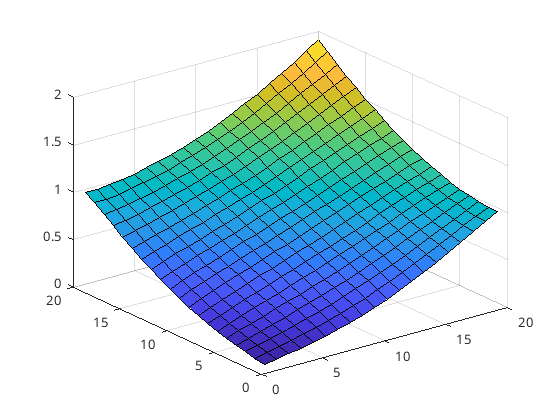
\includegraphics[width=0.5\textwidth]{img/5/homework_5_1.png}
    \caption{计算数据}
\end{figure}

对比预期结果:

\begin{figure}[h]
    \centering
    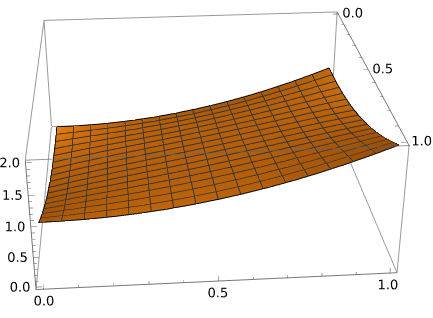
\includegraphics[width=0.5\textwidth]{img/5/homework_5_1_expected.png}
    \caption{预期结果}
\end{figure}

可以看到结果基本正确(截图的时候角度不太一致,下图旋转一下就能看出)。

\end{document}